\Chapter{Megvalósítás}


\section{Adatbázisok és modellek}
A programban a drón, és telemetria adatmodell a legfontosabb.
Ezeket az adatokat olvassuk és mentjük,illetve szükségesek az azonosításhoz vagy bármilyen értelmes következtetéshez a problémához kapcsolódóan.

\subsection{Modellek az adatközpont programban}
\subsubsection{Telemetria modell}
A programban a telemetria modell a következőképpen néz ki:
\begin{python}
    package models

    import "time"

    type Telemetry struct {
        Speed              float64          `json:"speed" db:"speed"`
        Location           GPS              `json:"location" `
        Altitude           float64          `json:"altitude" ` // in meters
        Bearing            float64          `json:"bearing" `
        Acceleration       float64          `json:"acceleration" `
        BatteryLevel       int              `json:"battery_level" `
        BatteryTemperature int              `json:"battery_temperature" `
        MotorTemperatures  []int            `json:"motor_temperatures" `
        Errors             []TelemetryError `json:"errors" db:"errors" `
        TimeStamp          time.Time        `json:"time_stamp" `
        DroneID            int              `json:"drone_id" `
    }

    type TelemetryError int

    const (
        MotorFailure TelemetryError = iota
        BeaconSignalStrengthLow
        BeaconSignalInterference
        BeaconTemperatureTooHigh
        GPSInteference
        GPSSignalLost
        GPSTemperatureTooHigh
        ProcessorTemperatureTooHigh
        BatteryFailure
        FailedToEjectPackage
        PackageLost
        DestinationDistanceTooFar
    )

    type GPS struct {
        Latitude  float64 `json:"latitude" bson:"latitude"`
        Longitude float64 `json:"longitude" bson:"longitude"`
    }

\end{python}


\subsubsection{Drone modell}
\begin{python}
    type Drone struct {
        ID           int           `json:"id" db:"drone_id" bson:"id"`
        Telemetry    Telemetry     `json:"telemetry" bson:"telemetry"`
        Parcel       Parcel        `json:"parcel"`
        Destinations []Destination `json:"destinations"`
        Consumption  float64       `json:"consumption"`
        Weight       float64       `json:"weight"`
        State        DroneState    `db:"state" bson:"state"`
    }

    type DroneState string

    const (
    DroneFree     DroneState = "free"
    DroneInFlight DroneState = "in-flight"
    )
\end{python}


\subsubsection{Parcel modell (szállítandó csomag)}
A drónok által szállított csomag így néz ki:
\begin{python}
    type Parcel struct {
        ID            int             `json:"id" db:"id" bson:"id"`
        TrackingID    string          `json:"tracking_id" `
        Name          string          `json:"name" db:"name" bson:"name"`
        Weight        float64         `json:"weight" db:"weight"`
        Location      GPS             `json:"location" bson:"location"`
        FromAddress   ShippingAddress `json:"from_address"`
        ToAddress     ShippingAddress `json:"to_address"`
        DropOffSite   GPS             `bson:"drop_off_site" `
        AssignedDrone int             `json:"assigned_drone" `
    }
\end{python}

\subsection{Relációs adatbázis, PostgreSQL modell}
A relációs adatbázissal is működik a szimuláció.
\paragraph{Relációs modell \ref{fig:postgres} } \mbox{} \\

\begin{figure}[h]
    \centering
    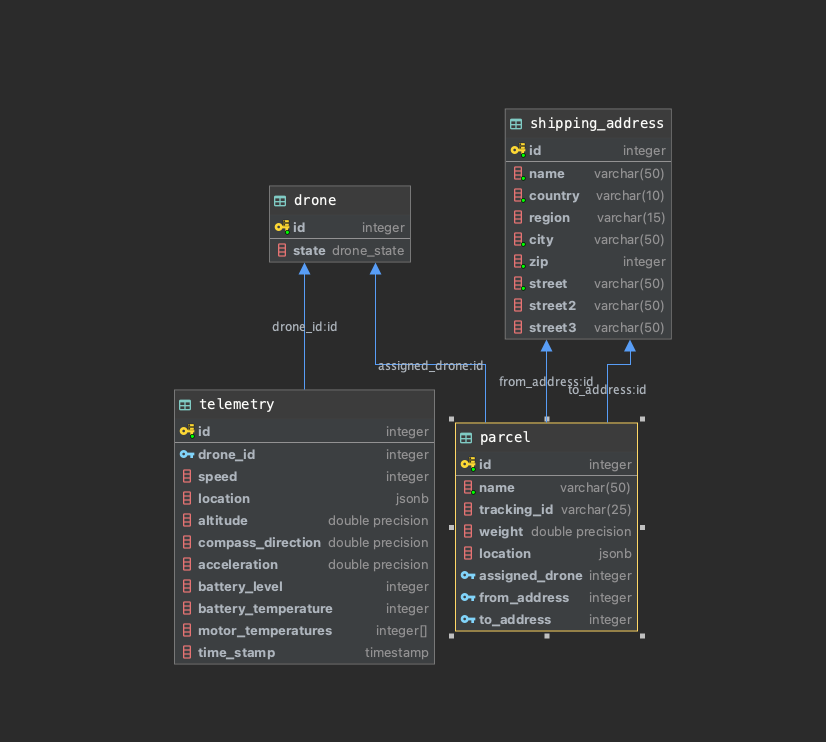
\includegraphics[scale=0.4]{images/postgres.png}
    \caption{PostgreSQL adatbázis modell}
    \label{fig:postgres}
\end{figure}

%TODO: ide táblázattal megcsinalni a relacios modellt


\paragraph{Lost Update probléma} \mbox{} \\
A legtöbb relációs adatbázis támogatja a tranzakciókat. A tranzakciók ACID tulajdonságokkal bírnak.
Adatbázisok esetén az ACID az Atomicity (atomiság), Consistency (konzisztencia), Isolation (izoláció), és Durability (tartósság) rövidítése. Ezek nélkül az adatbázis integritása nem garantálható.
A PostgreSQL többféle izolációs szintet biztosít a tranzakciókhoz \cite{postgres-transaction}. A Lost Update problémát garantáltan megoldja a PostgreSQL `Serializable` izolációs szintje.
\begin{table}[h]
    \centering
    \caption{ Standard SQL Transaction Isolation Levels}
    \begin{tabular}{l|c|c|c|}
Isolation Level & Dirty Read  & Nonrepeatable Read & Phantom Read\\
        \hline
Read uncommitted  & Possible & Possible & Possible \\
\hline
Read committed & Not possible & Possible & Possible \\
\hline
Repeatable read & Not possible & Not possible & Possible \\
\hline
Serializable & Not possible & Not possible & Not Possible \\
        \hline
    \end{tabular}
\end{table}

\subsection{Dokumentum alapú adatbázis, MongoDB}

A telepítéshez
\begin{python}
    use drone_delivery
\end{python}

\begin{python}

    db.createUser(
        {
        user: "drone-user",
        pwd: "drone-pwd",
        roles: [
            {
            role: "readWrite",
            db: "drone_delivery"
        }
        ]
    }
    )
\end{python}

\section{A réteges felépítés}
%TODO: ide irni
dsdas


\section{Számítási problémák}
A program implementálása közben gondot okozott, hogy a Föld alakját is figyelembe kell venni a repülésnél.
Ugyanis itt a Cartesian féle geometria nem jól működik, mivel a Földnek gömb alakja van.
Emiatt teljesen máshogy kell számolni távolságot.
\subsection{Cartesian szerinti}
\begin{gather}
    P_1(5,6,3) \\
    P_2(7,4,9) \\
    V = 10 \frac{m}{s}
\end{gather}


Kiszamitas:

\begin{gather}
    x = r * cos(\phi) * sin(\theta) \\
    y = r * sin(\phi) * sin(\theta) \\
    z = r * cos(\theta)
\end{gather}


X, Y, Z, r

\begin{gather}
    x = X_2 - X_1 = 7 - 5 = 2 \\
    y = Y_2 - Y_1 = 4 - 6 = -2 \\
    z = Z_2 - 7_1 = 9 - 3 = 6 \\
    r = \sqrt{2^2 + (-2)^2 + 6^2} = \sqrt{44}
\end{gather}

$
cos(\phi) sin(\phi) cos(\theta) sin(\theta)
$

\begin{gather}
    cos(\phi) = \frac{x}{\sqrt{x^2 + y^2}} \\
    sin(\phi) = \frac{y}{\sqrt{x^2 + y^2}} \\
    cos(\theta) = \frac{\sqrt(x^2 + y^2)}{\sqrt{x^2 + y^2 + z^2}} \\
    sin(\theta) = \frac{z}{\sqrt{x^2 + y^2 + z^2}}
\end{gather}

\newpage

További számítás segédvektorok kiszámítása:

\begin{gather}
    V_x = \frac{x}{\sqrt{x^2 + y^2 + z^2}} *V = \frac{2}{\sqrt{44}} * 10 = \frac{10\sqrt{11}}{11} = 3.0151\\
    V_y = \frac{y}{\sqrt{x^2 + y^2 + z^2}} *V = \frac{-2}{\sqrt{44}} * 10 = -\frac{10\sqrt{11}}{11} = -3.0151\\\\
    V_z = \frac{z}{\sqrt{x^2 + y^2 + z^2}} *V = \frac{6}{\sqrt{44}} * 10 = \frac{30\sqrt{11}}{11} = 9.0453\\
\end{gather}

Összesen eltelt idő:

\begin{gather}
    t = \frac{s}{v}
\end{gather}

\begin{gather}
    t_osszes = \frac{\sqrt{(x_2 - x_1)^2 + (y_2 - y_1)^2 + (z_2 - z_1)^2}}{v} = \frac{\sqrt{(7 - 5)^2 + (4 - 6)^2 + (9 - 3)^2}}{10} = \frac{\sqrt{44}}{10}{}
\end{gather}

t idő múlva egy adott pillanatban koordináták meghatározása:

\begin{gather}
    x = X_0 + V_x * t = X_0 + \frac{X}{\sqrt{x^2 + y^2 + z^2}} * t = 5 + \frac{2}{\sqrt{44}} * 10 * t \\
    Y = y_0 + V_y * t = y_0 + \frac{y}{\sqrt{x^2 + y^2 + z^2}} * t = 4 - \frac{2}{\sqrt{44}} * 10 * t \\
    z = z_0 + V_z * t = z_0 + \frac{z}{\sqrt{x^2 + y^2 + z^2}} * t = 6 + \frac{6}{\sqrt{44}} * 10 * t
\end{gather}

\subsection{Az Ortodroma számítás, a föld alakját figyelembe véve}

Mivel gömbi geometria lényegesen eltér az euklideszi geometriától ezért a távolságszámításra használt matematikai képletek is eltérőek.
Az euklideszi geometriában a legrövidebb távolságot a két pontot összekötő egyenes,
a nem euklideszi geometriában a két pontot összekötő geodetikus vonal (gömb esetén főkör) mentén mérjük.

\paragraph{A legrövidebb út kiszámítása}
\begin{gather}
    d = arccos(sin\phi_1 * sin\phi_2 * cos\phi_1)* cos\phi_2 * cos\Delta \lambda) * R
\end{gather}

\paragraph{Irány kiszámítása}
Ahogy az főkörön haladunk az irányunk folyamatosan változik. Tehát amikor megérkezünk a célhoz, nem ugyanabban az irányba nézünk mint amikor elindultunk.
A drón szimulációban ez a telemetria adatokban is megfigyelhető.
\begin{gather*}
    \varphi = atan2(sin\Delta\lambda * cos\phi_{2}, cos\phi_{1} * sin\phi_{2} - sin\phi_{1} * cos\phi_{2} * cos\Delta\lambda)
\end{gather*}
ahol $\phi_{1}\lambda_{1}$ a kezdeti pont, és $\phi_{2}\lambda_{2}$ a vég pont és $\Delta\lambda$ pedig a különbség a hosszúsági fokokban.

\paragraph{Cél koordináták kiszámítása, ha ismerjük a megtett távolságot, irányt, és kezdő koordinátákat}
\begin{gather}
    \phi_{2} = arcsin(sin \phi_{1} * cos \delta + cos \phi_{1} * sin \delta * cos \theta)\\
    \lambda_{2} = \lambda_{1} + arctan2(sin\theta * sin\delta  * cos\phi_{1}, cos\delta - sin\phi_{1} * sin\phi_{2})
\end{gather}
ahol $\phi$ a szélességi fok, $\lambda$ a hosszúsági fok, $\theta$ az irány, $\delta$ a szögtávolság d/R és d a megtett távolság, R pedig a Föld sugara.

\subsection{Megvalósítás a programban}
\subsubsection{Az adatközpont távolság számítása}
Az adatközpont program az Ortodroma számítást használja, hogy kiszámolj a távolságot a legoptimálisabb útvonal keresése közben.
Ez a számítás nem tökéletes, nem ér fel egy nagyon pontos GPS rendszerrel de a problémát tökéletesen megoldja.
\begin{python}
    func (s *service) CalculateDistance(lat1, lng1, lat2, lng2 float64, unit ...string) float64 {
        const PI = float64(math.Pi) //3.141592653589793

        radlat1 := PI * lat1 / 180
        radlat2 := PI * lat2 / 180

        theta := lng1 - lng2
        radtheta := PI * theta / 180

        dist := math.Sin(radlat1)*math.Sin(radlat2) + math.Cos(radlat1)*math.Cos(radlat2)*math.Cos(radtheta)

        if dist > 1 {
            dist = 1
        }

        dist = math.Acos(dist)
        dist = dist * 180 / PI
        dist = dist * 60 * 1.1515

        if len(unit) > 0 {
            if unit[0] == "K" {
                dist = dist * 1.609344
            } else if unit[0] == "N" {
                dist = dist * 0.8684
            } else if unit[0] == "METER" {
                dist = dist * 1.609344 * 1000
            }
        }

        return dist
    }
\end{python}
\subsubsection{A drón-raj program számításai}
A pontos szimulációs értékekhez egy sokkal komolyabb könyvtárat használunk, ami megfelel a WGS84 GPS rendszernek.
Ezzel a könyvtárral pontos adatokat tudunk generálni a drón helyzetéről, irányáról.


\begin{python}
\end{python}


%TODO: Még ide kell a Go-kit, azért lett ez választva mert nem framework, hanem egy library/ecosystem, így több szabadságot kap a program,
%hogy hogyan is lesz mikroszerviz. Go kit ben van service discovery,  beepitett Observability (Prometheus), többszintes logger, és A hexagonal architektúrát támogatja
%Pl más hasonló mikroszervizeket kezelő framework (pl. Micro) nem elég rugalmas, sok mindent nem enged meg, egy féleképpen lehet használni.
